\documentclass{beamer}

\usepackage[utf8x]{inputenc}
\usepackage[OT4]{fontenc}

\usetheme[bullet=circle,
          titleline=true,
          pageofpages=z,
          alternativetitlepage=true]{Torino}

\usepackage{ragged2e}
\usepackage{hyphenat}
\usepackage{hyperref}
\usepackage{booktabs}

\usepackage{pgf,tikz}
\usepackage{pgfplots}

\usetikzlibrary{arrows}
\usetikzlibrary{automata}
\usetikzlibrary{backgrounds}
\usetikzlibrary{decorations}

\usepackage{amsmath}
\usepackage{amsfonts}
\usepackage{amsthm}

\title{
    Design and implementation issues \newline
    of a computer algebra system \newline
    in an interpreted, dynamically typed \newline
    programming language
}

\author{Mateusz Paprocki \texttt{<mattpap@gmail.com>}}
\institute[PWR]{Wrocław University of Technology}
\date{\today}

\newenvironment{jblock}[1]{
    \begin{block}{#1}\justifying\nohyphens
}{
    \end{block}
}

\setbeamercovered{transparent}

\begin{document}

\frame{\titlepage}

\begin{frame}
    \frametitle{}
    \framesubtitle{}

    \begin{center}
        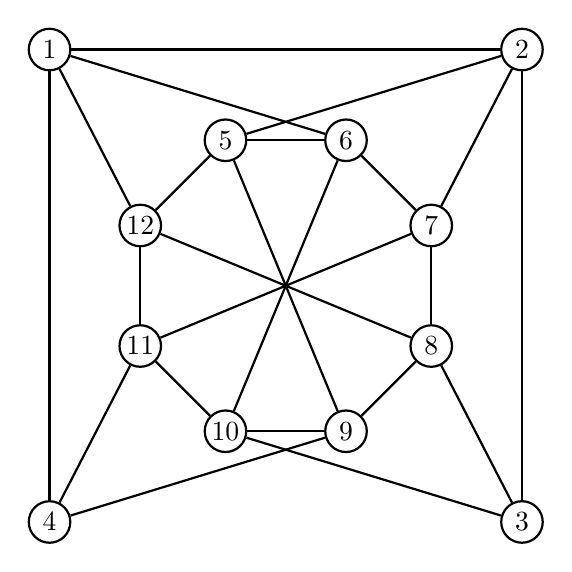
\begin{tikzpicture}[scale=2]
            \tikzstyle{edge}=[draw=black,thick,-]
            \tikzstyle{node}=[circle,thick,draw=black,fill=white,minimum size=15pt,inner sep=0pt]

            \def\x{0.382683}
            \def\y{0.923879}

            \def\z{1.5}

            \node[node] (x1)  at (-\z, \z) {$1$};
            \node[node] (x2)  at ( \z, \z) {$2$};
            \node[node] (x3)  at ( \z,-\z) {$3$};
            \node[node] (x4)  at (-\z,-\z) {$4$};
            \node[node] (x5)  at (-\x, \y) {$5$};
            \node[node] (x6)  at ( \x, \y) {$6$};
            \node[node] (x7)  at ( \y, \x) {$7$};
            \node[node] (x8)  at ( \y,-\x) {$8$};
            \node[node] (x9)  at ( \x,-\y) {$9$};
            \node[node] (x10) at (-\x,-\y) {$10$};
            \node[node] (x11) at (-\y,-\x) {$11$};
            \node[node] (x12) at (-\y, \x) {$12$};

            \path[edge] (x1) -- (x2);
            \path[edge] (x1) -- (x4);
            \path[edge] (x1) -- (x6);
            \path[edge] (x1) -- (x12);

            \path[edge] (x2) -- (x3);
            \path[edge] (x2) -- (x5);
            \path[edge] (x2) -- (x7);

            \path[edge] (x3) -- (x8);
            \path[edge] (x3) -- (x10);

            \path[edge] (x4) -- (x9);
            \path[edge] (x4) -- (x11);

            \path[edge] (x5) -- (x6);
            \path[edge] (x6) -- (x7);
            \path[edge] (x7) -- (x8);
            \path[edge] (x8) -- (x9);
            \path[edge] (x9) -- (x10);
            \path[edge] (x10) -- (x11);
            \path[edge] (x11) -- (x12);
            \path[edge] (x12) -- (x5);

            \path[edge] (x5) -- (x9);
            \path[edge] (x6) -- (x10);
            \path[edge] (x7) -- (x11);
            \path[edge] (x8) -- (x12);
        \end{tikzpicture}
    \end{center}
\end{frame}

\begin{frame}
    \frametitle{}
    \framesubtitle{}

    \begin{center}
        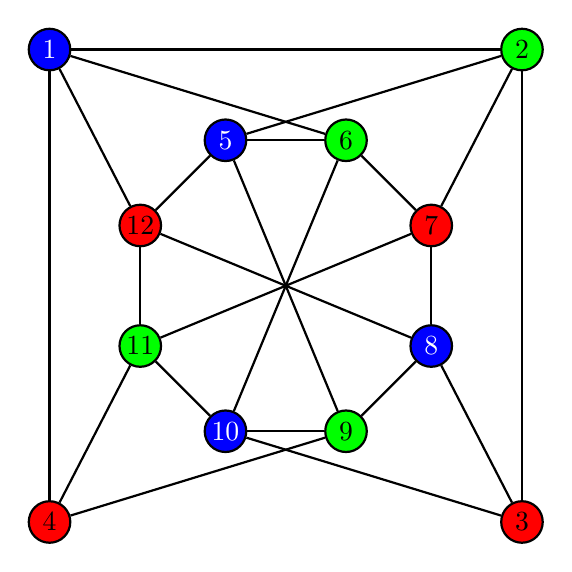
\begin{tikzpicture}[scale=2]
            \tikzstyle{edge}=[draw=black,thick,-]
            \tikzstyle{node}=[circle,thick,draw=black,fill=white,minimum size=15pt,inner sep=0pt]

            \tikzstyle{red}=[text=black,fill=red]
            \tikzstyle{green}=[text=black,fill=green]
            \tikzstyle{blue}=[text=white,fill=blue]

            \def\x{0.382683}
            \def\y{0.923879}

            \def\z{1.5}

            \node[node,blue]  (x1)  at (-\z, \z) {$1$};
            \node[node,green] (x2)  at ( \z, \z) {$2$};
            \node[node,red]   (x3)  at ( \z,-\z) {$3$};
            \node[node,red]   (x4)  at (-\z,-\z) {$4$};
            \node[node,blue]  (x5)  at (-\x, \y) {$5$};
            \node[node,green] (x6)  at ( \x, \y) {$6$};
            \node[node,red]   (x7)  at ( \y, \x) {$7$};
            \node[node,blue]  (x8)  at ( \y,-\x) {$8$};
            \node[node,green] (x9)  at ( \x,-\y) {$9$};
            \node[node,blue]  (x10) at (-\x,-\y) {$10$};
            \node[node,green] (x11) at (-\y,-\x) {$11$};
            \node[node,red]   (x12) at (-\y, \x) {$12$};

            \path[edge] (x1) -- (x2);
            \path[edge] (x1) -- (x4);
            \path[edge] (x1) -- (x6);
            \path[edge] (x1) -- (x12);

            \path[edge] (x2) -- (x3);
            \path[edge] (x2) -- (x5);
            \path[edge] (x2) -- (x7);

            \path[edge] (x3) -- (x8);
            \path[edge] (x3) -- (x10);

            \path[edge] (x4) -- (x9);
            \path[edge] (x4) -- (x11);

            \path[edge] (x5) -- (x6);
            \path[edge] (x6) -- (x7);
            \path[edge] (x7) -- (x8);
            \path[edge] (x8) -- (x9);
            \path[edge] (x9) -- (x10);
            \path[edge] (x10) -- (x11);
            \path[edge] (x11) -- (x12);
            \path[edge] (x12) -- (x5);

            \path[edge] (x5) -- (x9);
            \path[edge] (x6) -- (x10);
            \path[edge] (x7) -- (x11);
            \path[edge] (x8) -- (x12);
        \end{tikzpicture}
    \end{center}
\end{frame}

\end{document}

